%%%%%%%%%%%%%%%%%%%%%%%%%%%%%%%%%%%%%%%%%%%%%%%%%%%%%%%%%%%%%%%%%%%%%%%%%%%

\documentclass{standalone}

\usepackage{amsmath}
\usepackage{mathptmx}
\usepackage{pgfplots}
\usetikzlibrary{external}
\tikzexternalize{e-12-growth-factor}
\pgfplotsset{compat=1.16}

%% IEEE uses Times Roman font, so we'll default to Times.
%% These three commands make up the entire times.sty package.
\renewcommand{\rmdefault}{ptm}
\renewcommand{\ttdefault}{pcr}
\normalfont\selectfont

\begin{document}

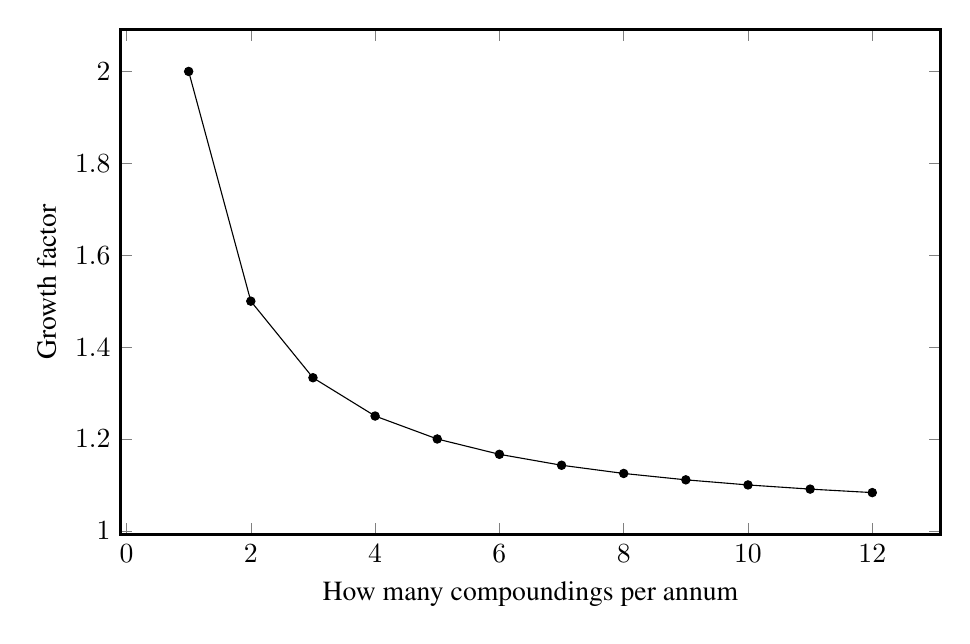
\begin{tikzpicture}
\tikzset{%%
  every mark/.append style={scale=1.0},%%
  scale=1.0%%
}
\pgfplotsset{%%
  every axis/.append style={font=\normalsize}%%
}
%%
\begin{axis}[%%
  axis line style=very thick,%%
  dotStyle/.style={mark size=1.5,black,mark color=black,mark=*},%%
  enlargelimits=true,%%
  height=8cm,%%
  width=12cm,%%
  %% x axis
  xlabel={\normalsize How many compoundings per annum},%%
  %% y axis
  ylabel={\normalsize Growth factor}%%
]
%%
%%
\addplot[dotStyle] coordinates {
  (1, 2)
  (2, 1.5)
  (3, 1.33333333333333)
  (4, 1.25)
  (5, 1.2)
  (6, 1.16666666666667)
  (7, 1.14285714285714)
  (8, 1.125)
  (9, 1.11111111111111)
  (10, 1.1)
  (11, 1.09090909090909)
  (12, 1.08333333333333)
};
\end{axis}
\end{tikzpicture}

\end{document}
